\documentclass[UTF8]{ctexart}
\usepackage{geometry}
\usepackage{amsmath}
\usepackage{graphicx} %插入图片的宏包
\usepackage{float} %设置图片浮动位置的宏包
\usepackage{setspace}
\geometry{a4paper,scale=0.8}
\sectionfont{\bfseries\Large\raggedright}

\title{3d影像显示报告}
\author{徐世桐}
\date{}
\begin{document}
\maketitle

% ----------------------------------------------------------------------
% |                               程序目标                               |
% ----------------------------------------------------------------------
\section{程序目标}
在终端内显示旋转的3d圆环。圆环的明亮处,阴影用不同字符表示。通过不断刷新输出字符显示动态的圆环旋转。程序运行效果截图如下:\\

\begin{figure}[htbp]
  \centering
  \begin{minipage}[t]{0.48\textwidth}
    \centering
    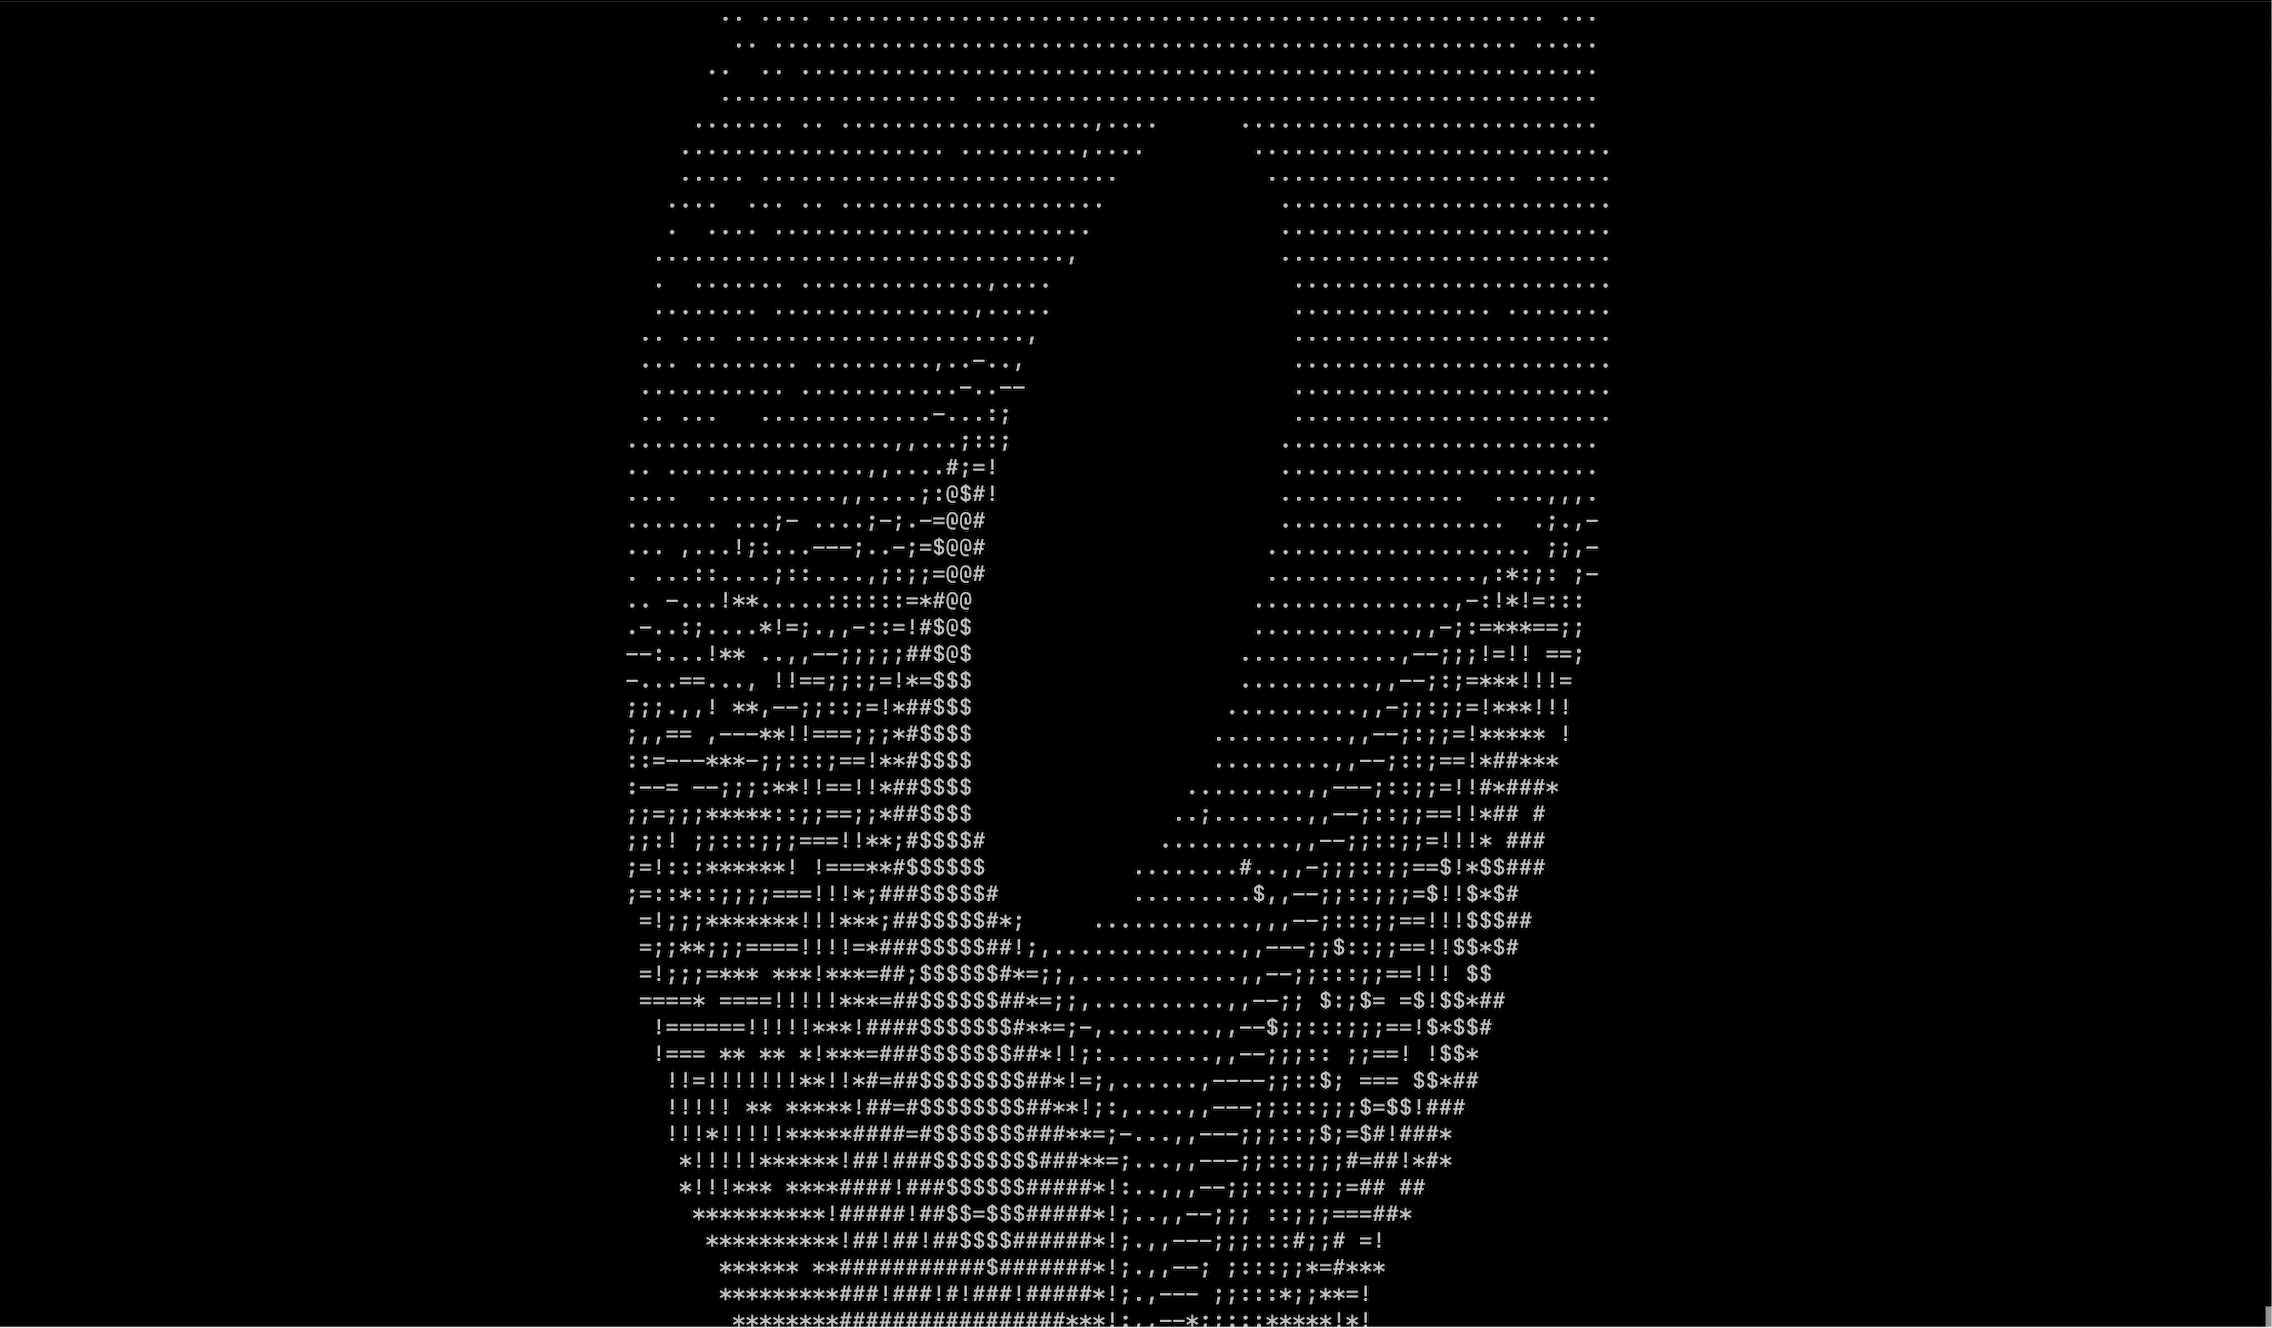
\includegraphics[width=6cm]{images/donout1.png}
  \end{minipage}
  \begin{minipage}[t]{0.48\textwidth}
    \centering
    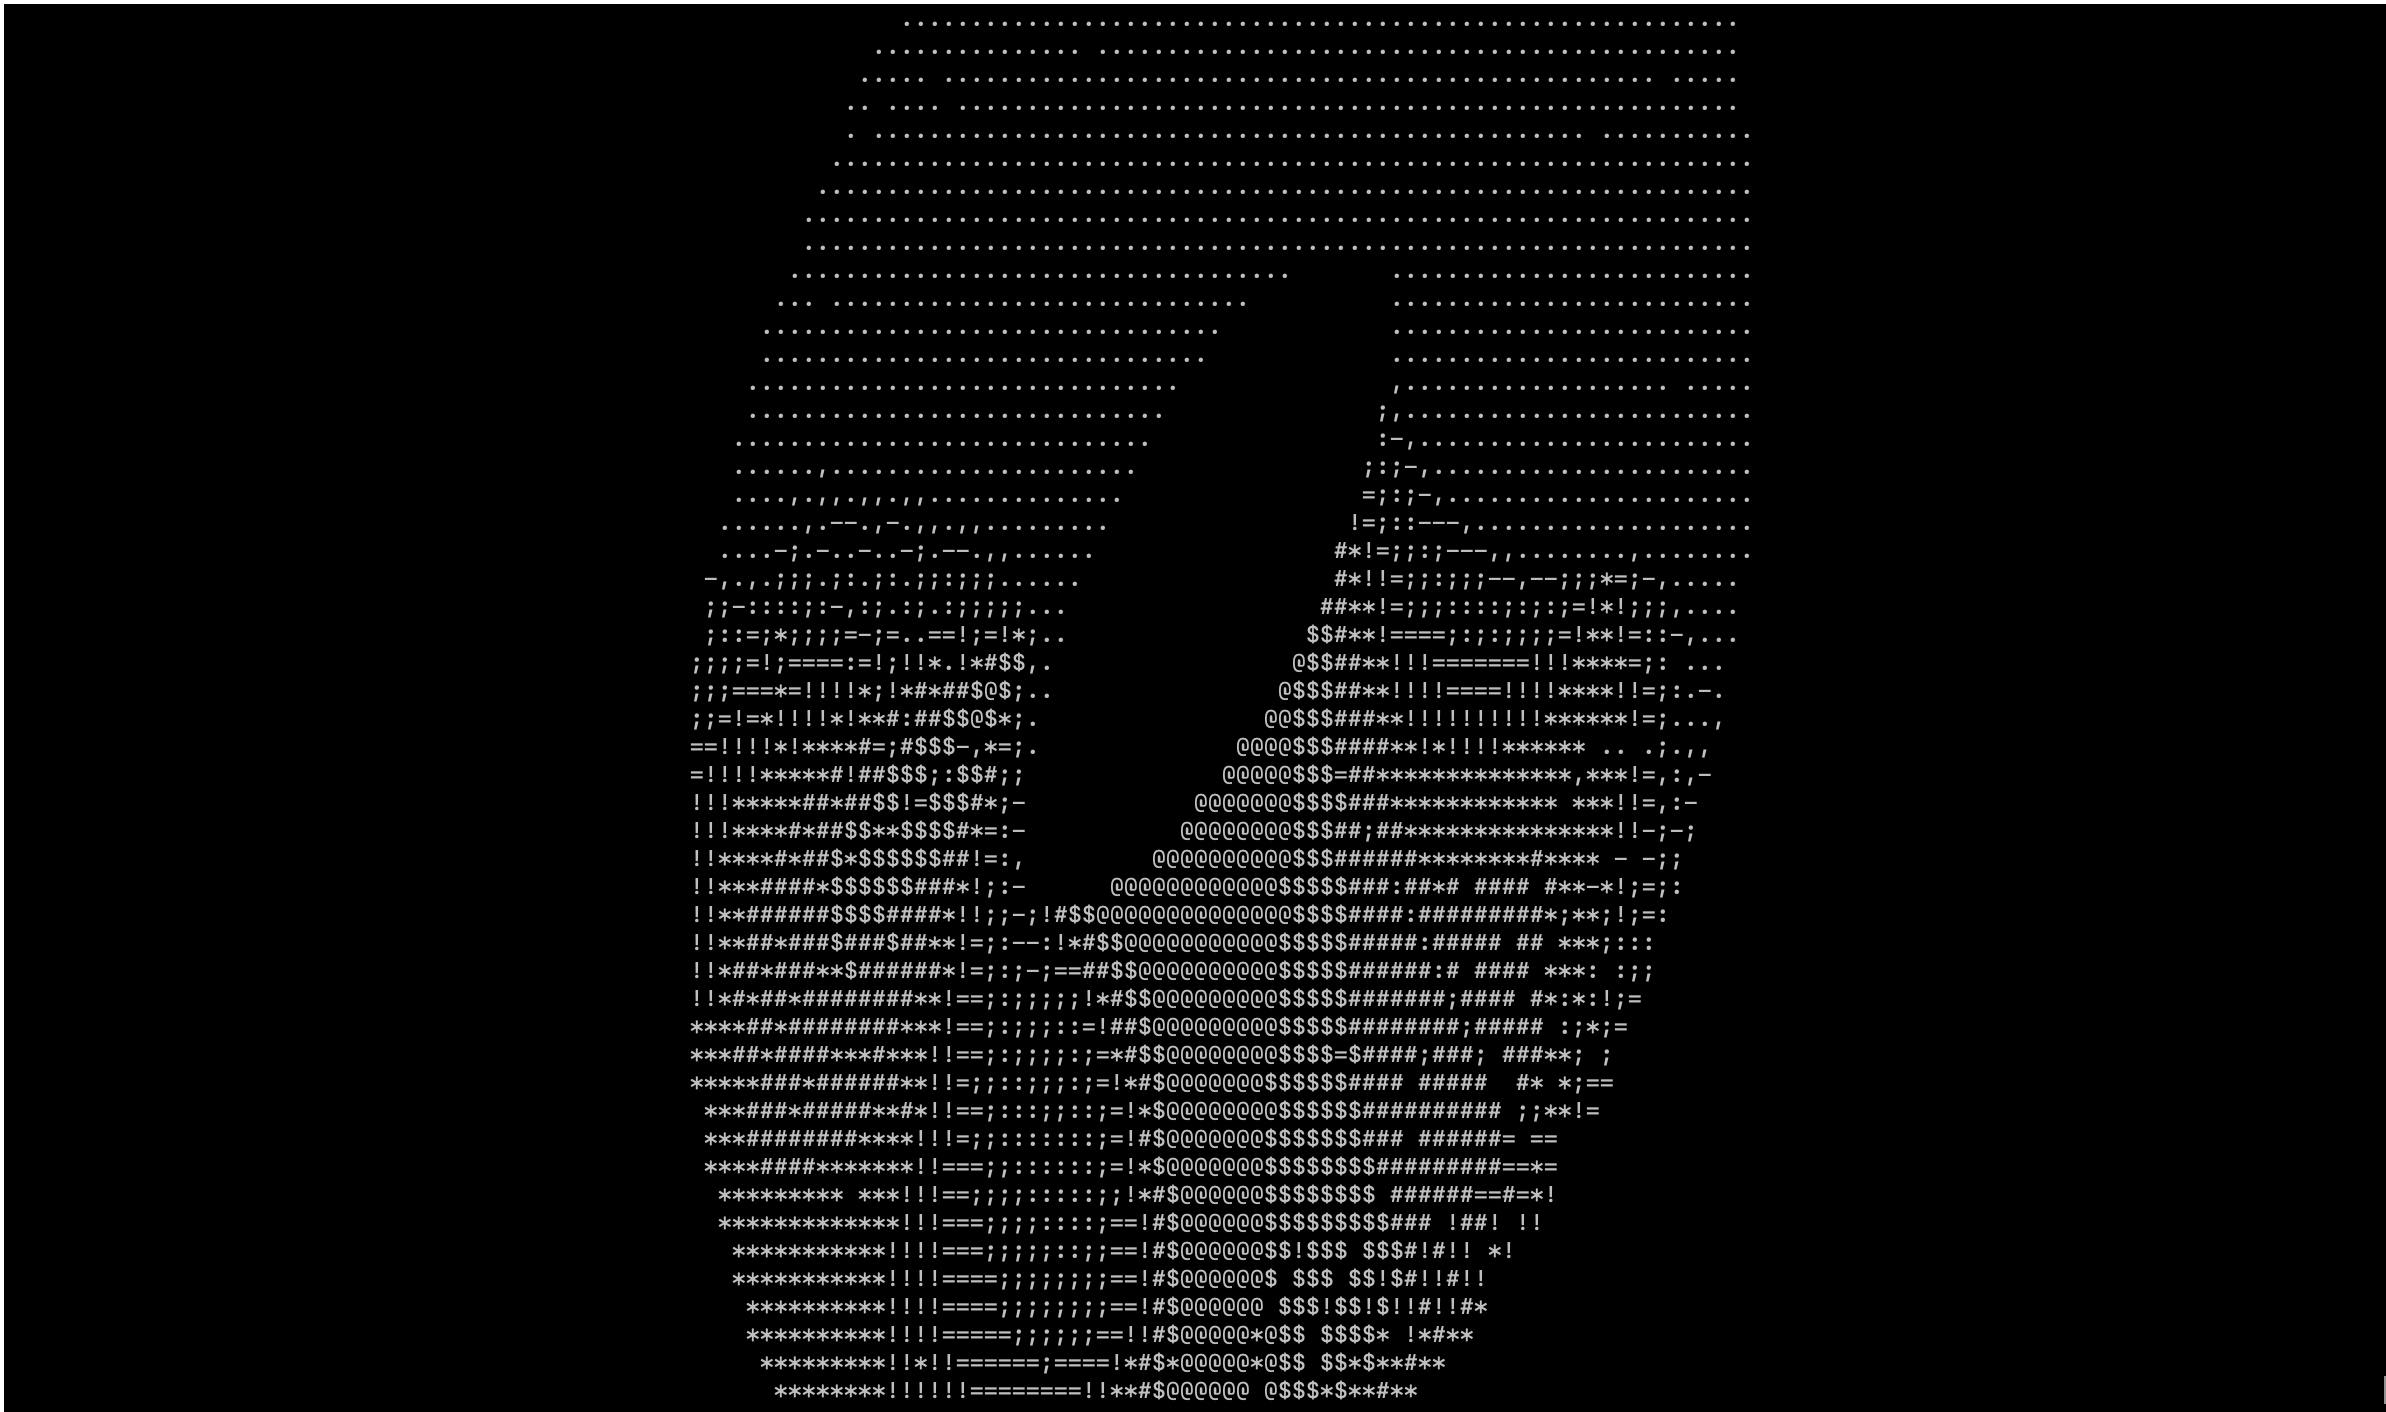
\includegraphics[width=6cm]{images/donout2.png}
  \end{minipage}
\end{figure}

\begin{figure}[htbp]
  \centering
  \begin{minipage}[t]{0.48\textwidth}
    \centering
    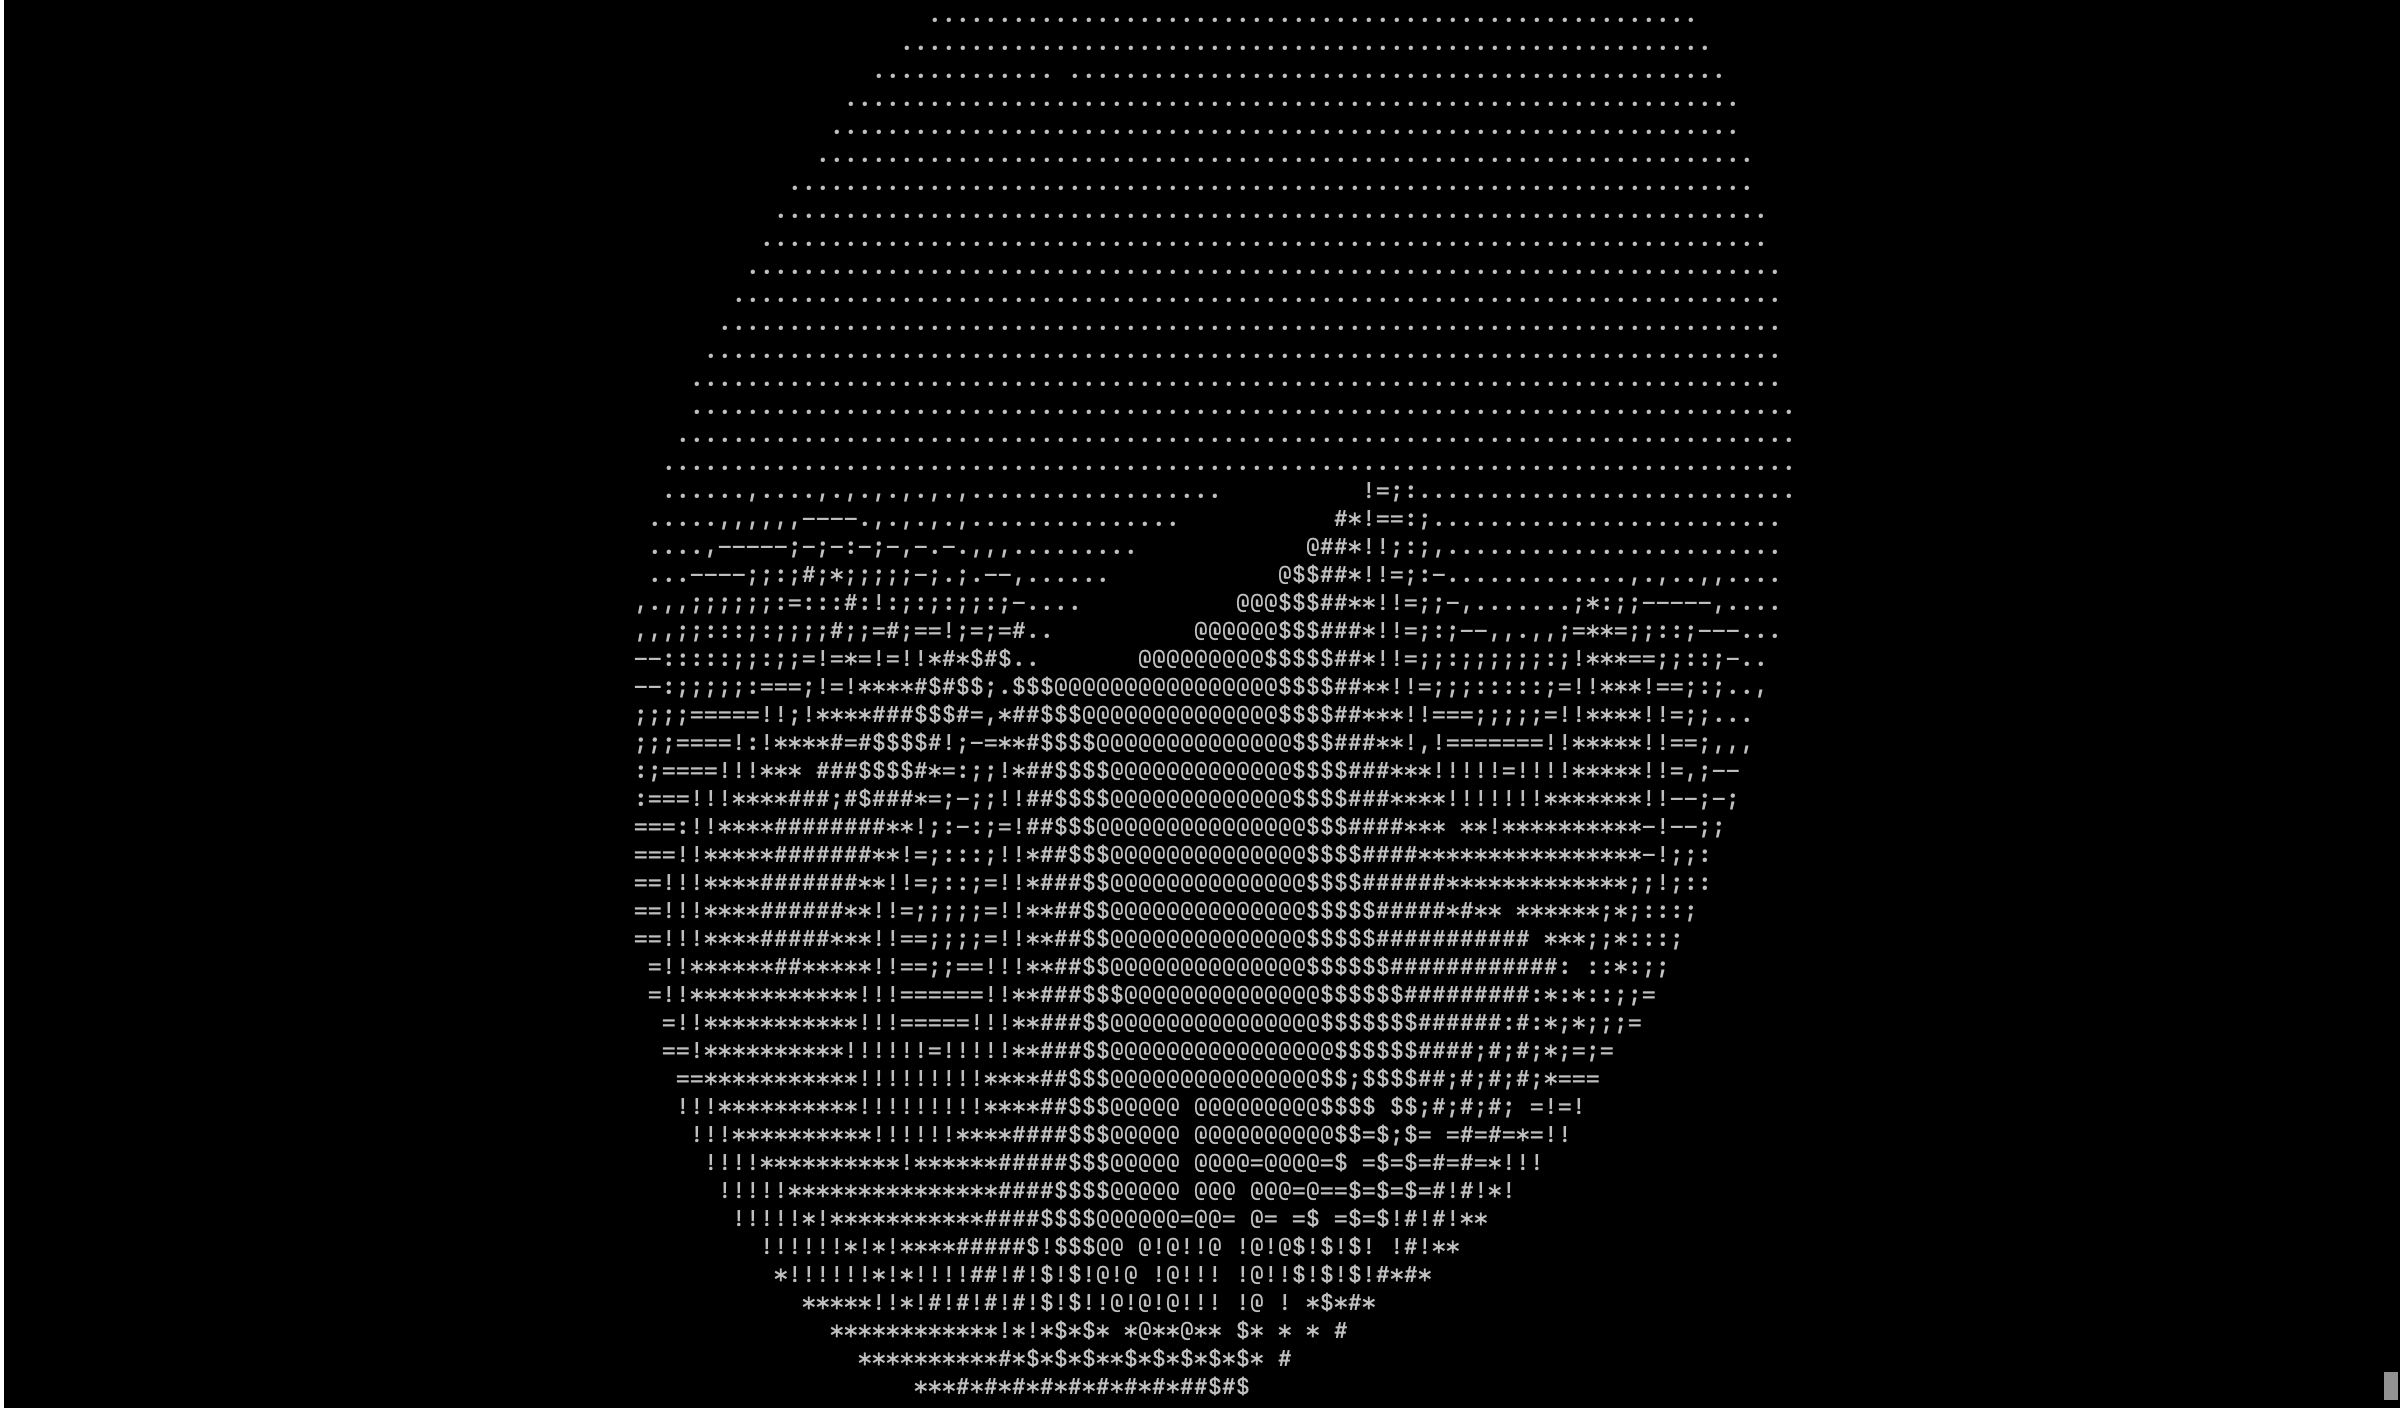
\includegraphics[width=6cm]{images/donout3.png}
  \end{minipage}
  \begin{minipage}[t]{0.48\textwidth}
    \centering
    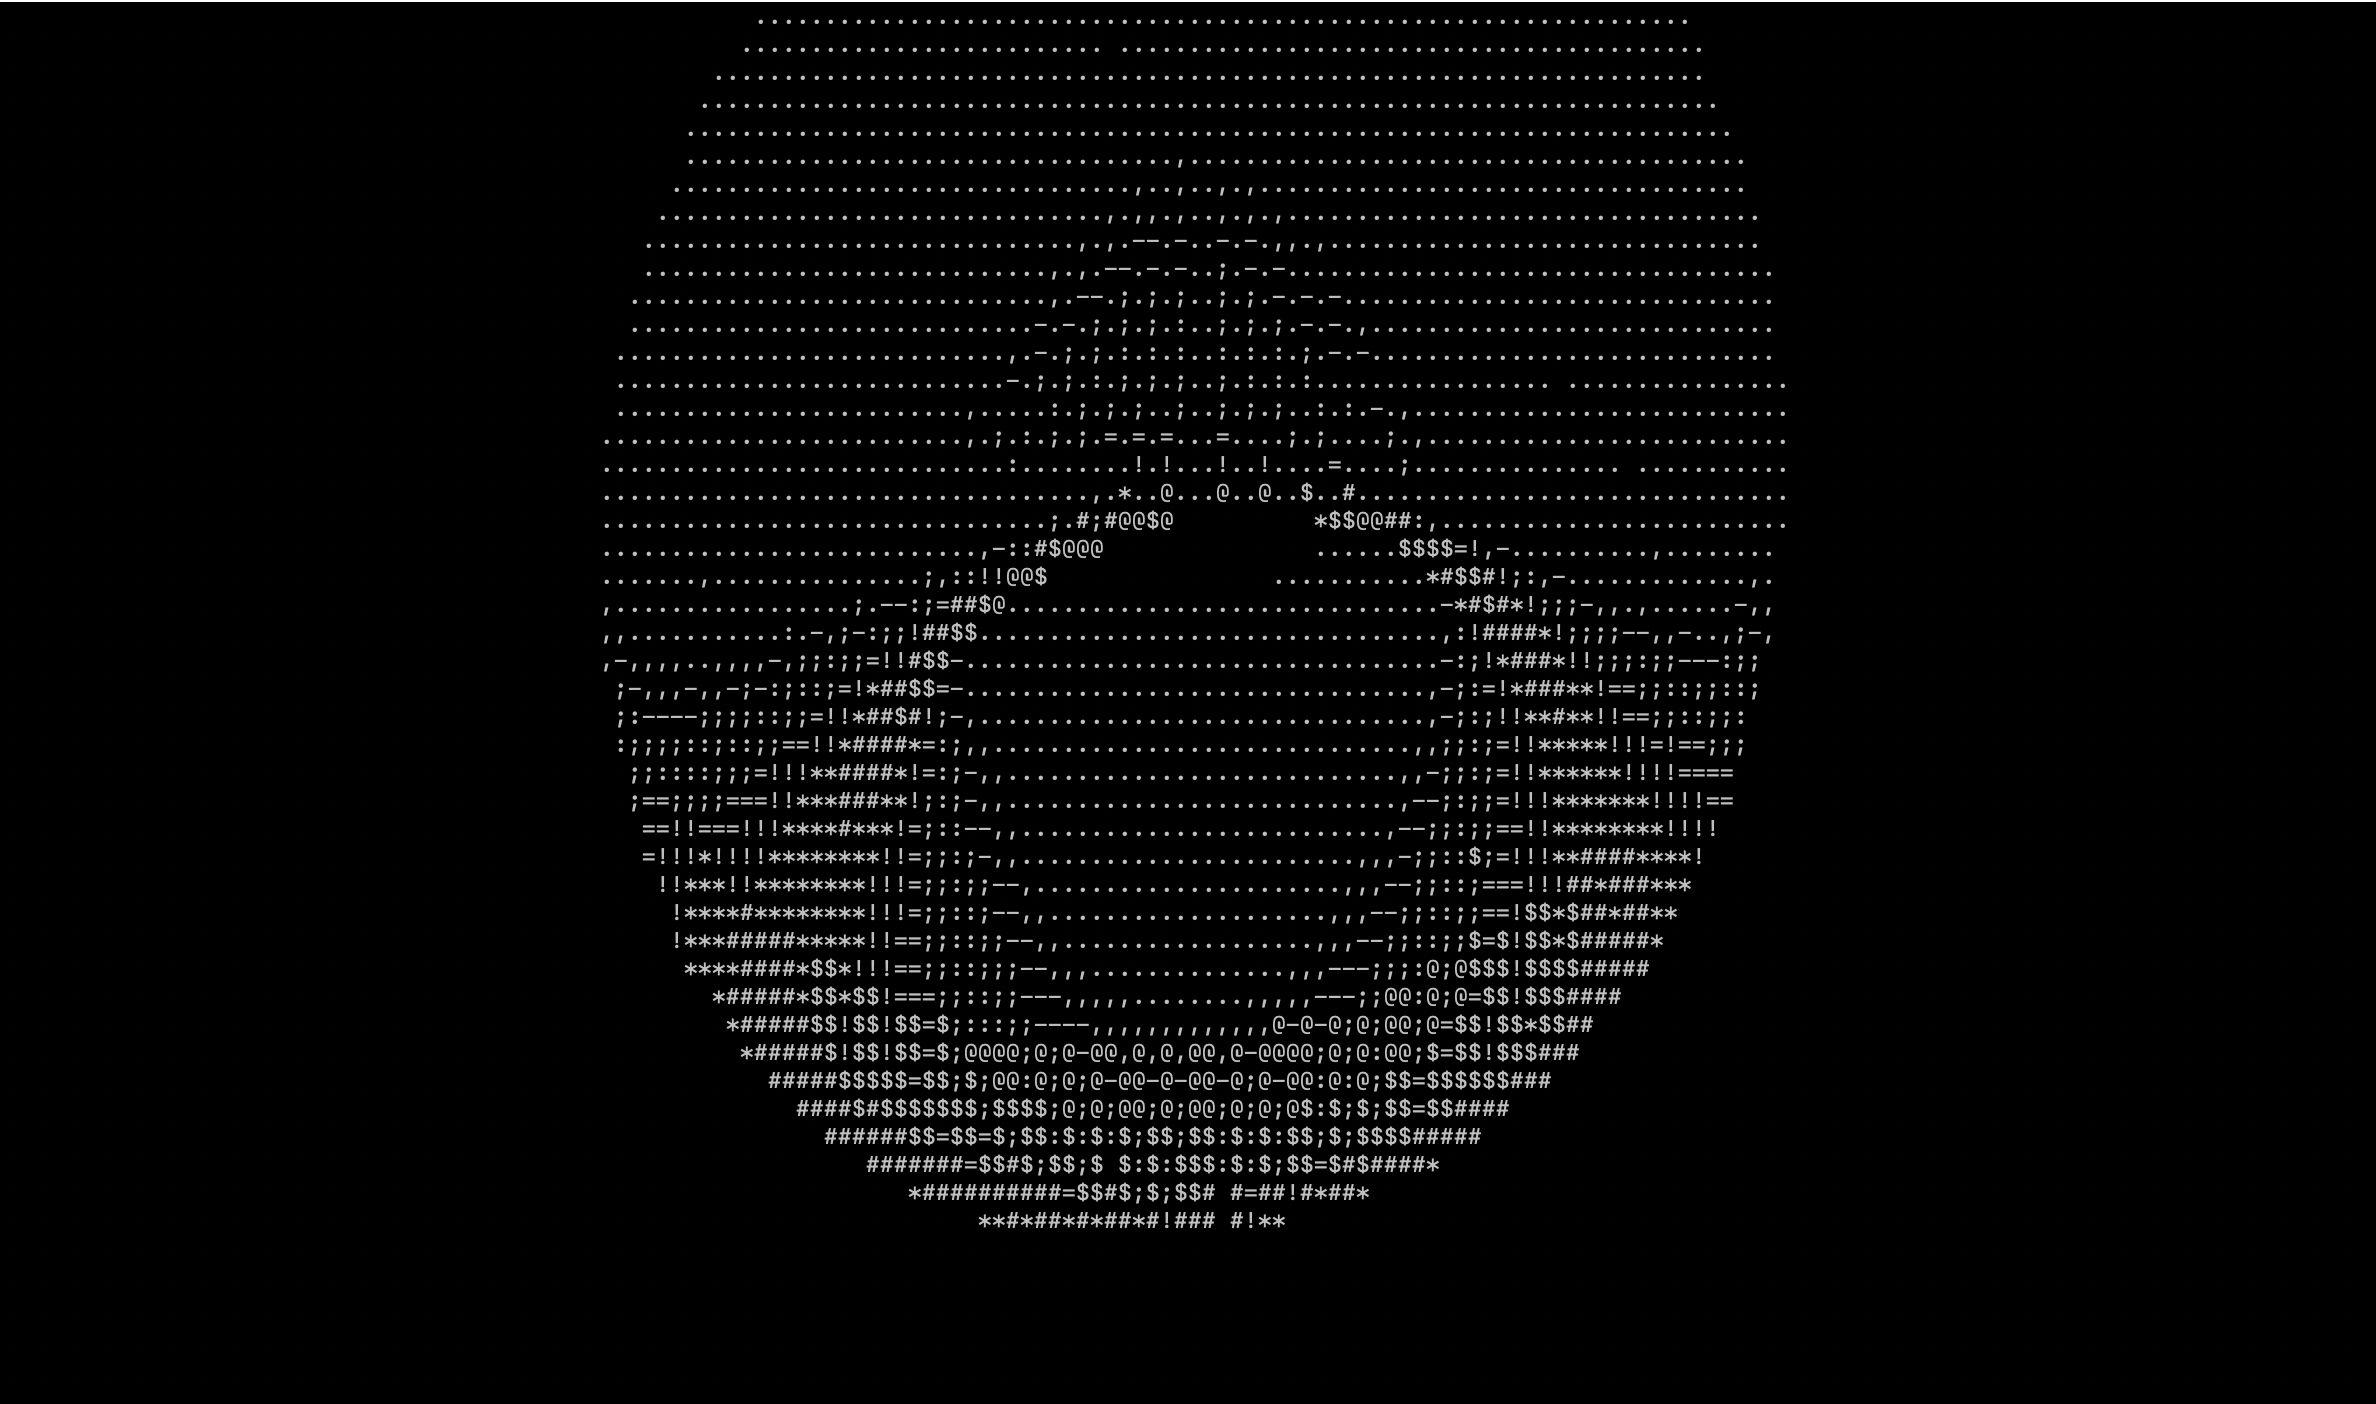
\includegraphics[width=6cm]{images/donout4.png}
  \end{minipage}
\end{figure}

程序想法来源于[1]

% ----------------------------------------------------------------------
% |                               功能实现                               |
% ----------------------------------------------------------------------
\section{功能实现}

整个程序分为:

\quad 1.从圆环的公式得到圆环上离散的点的坐标。

\quad 2.将圆环上每一点映射到二维画布上。

\quad 3.得到每一圆环上点的亮度。

\qaud 4.更新终端图片输出。

\quad 5.翻转圆环,回到第2步重新将圆环映射到二维平面,得到亮度,刷新显示

\subsection{圆环取点}

1.在x-y平面生成一个圆心在(100, 0, 0),半径为40的圆。
\begin{figure}[H] %H为当前位置,!htb为忽略美学标准,htbp为浮动图形
  \centering %图片居中
  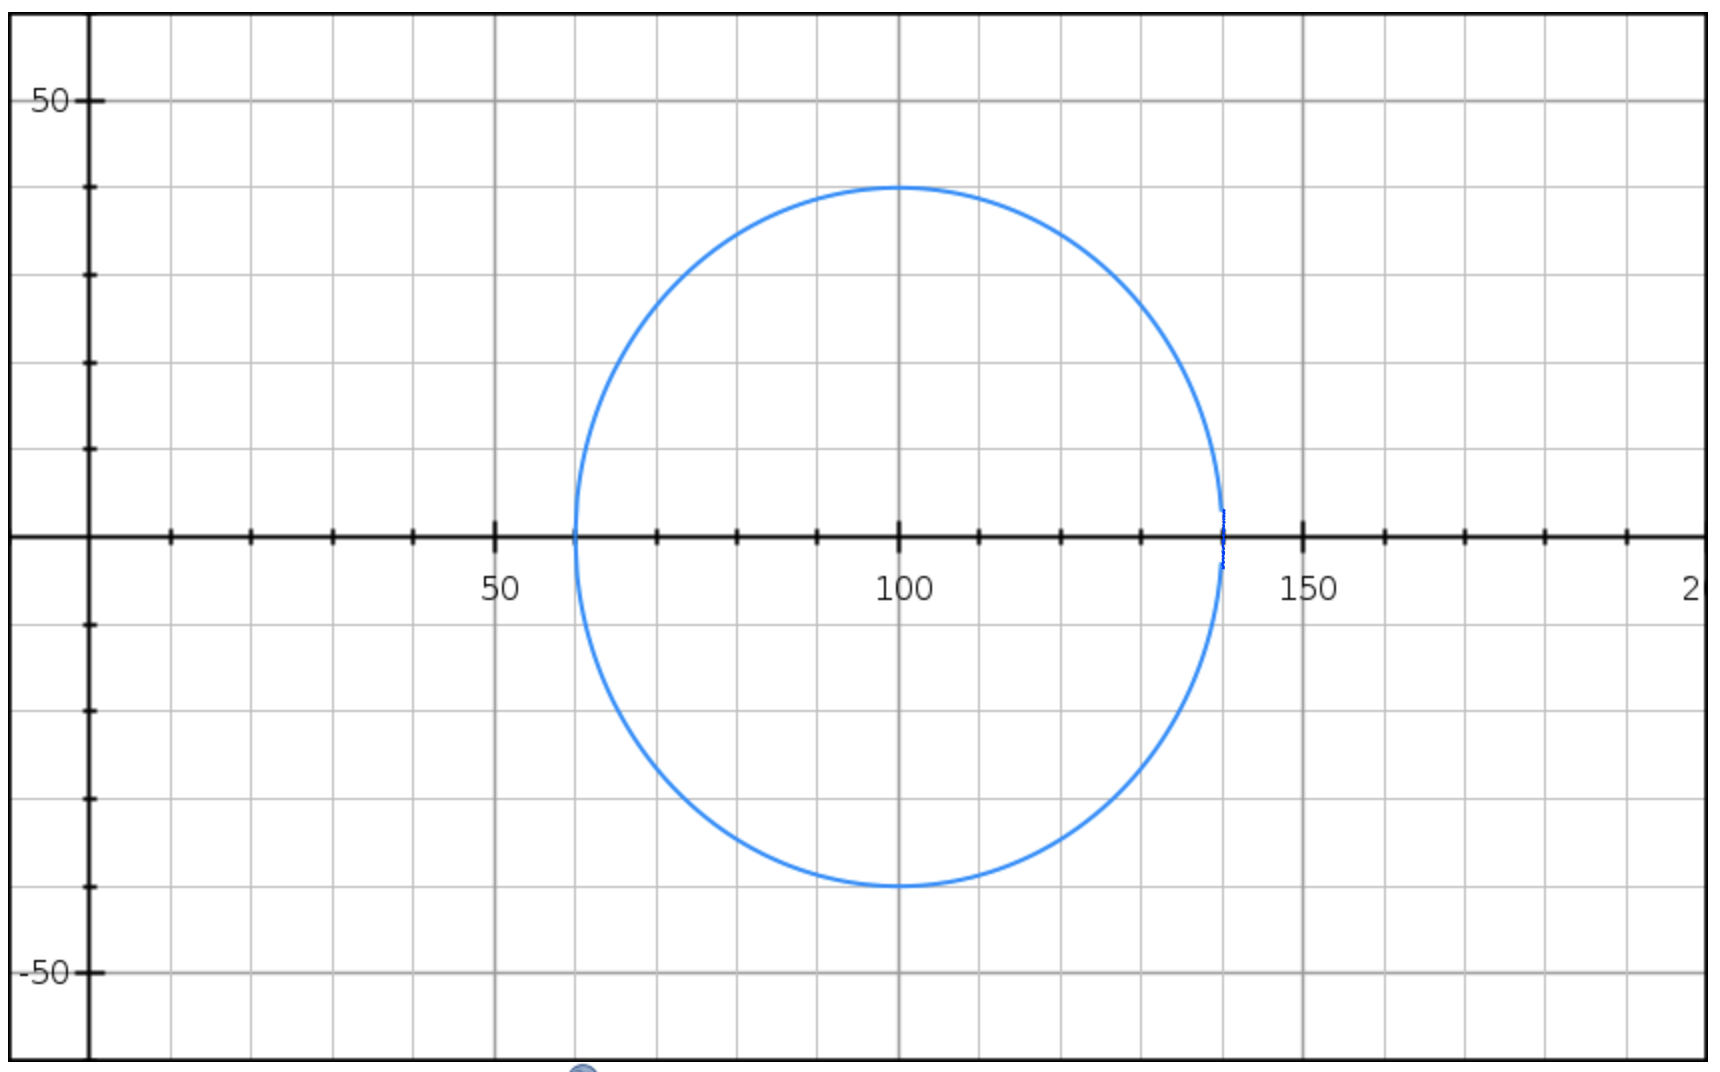
\includegraphics[width=0.3\textwidth]{images/2d-circle.png} %插入图片,[]中设置图片大小,{}中是图片文件名
\end{figure}

2.将圆沿y轴旋转,生成一个中心在(0, 0, 0)坐标原点的圆环,圆环截面即为1.中生成的圆。1.中圆上的点划出的轨迹如下图:
\begin{figure}[H] %H为当前位置,!htb为忽略美学标准,htbp为浮动图形
  \centering %图片居中
  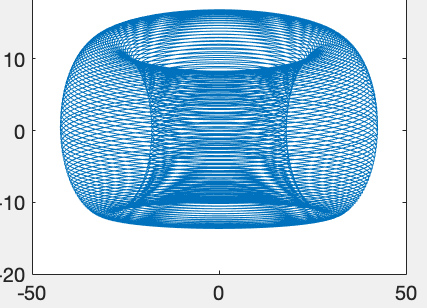
\includegraphics[width=0.3\textwidth]{images/3d-donout.png} %插入图片,[]中设置图片大小,{}中是图片文件名
\end{figure}

3.将圆环移动到中心位置为(0, 100, 1000)处,此步是为了方便将原点作为视线出发点,将圆环映射到二维平面。

\subsection{映射二维平面}

程序将圆环投影到位于z = 300,长170宽50的画布上。
\begin{figure}[H] %H为当前位置,!htb为忽略美学标准,htbp为浮动图形
  \centering %图片居中
  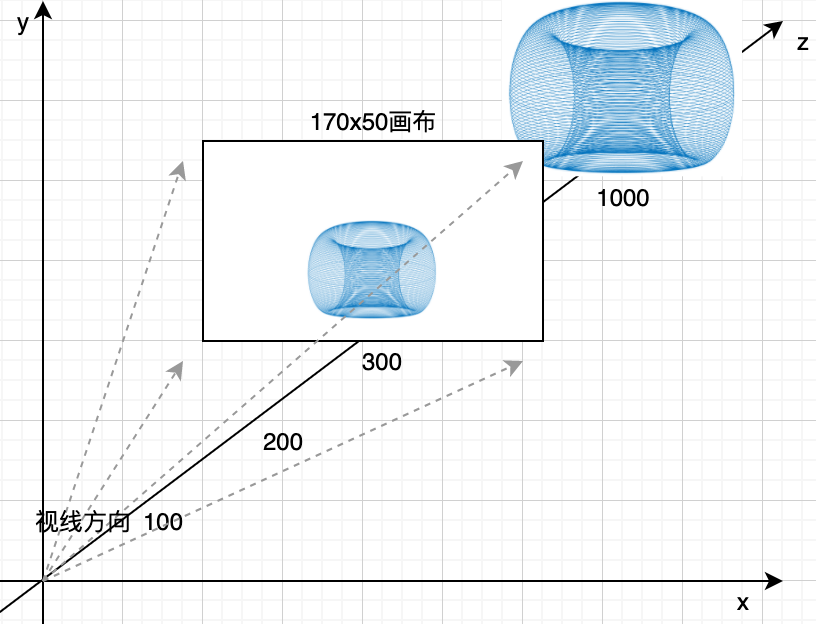
\includegraphics[width=0.3\textwidth]{images/canvas_view.png} %插入图片,[]中设置图片大小,{}中是图片文件名
\end{figure}

投影使用透视投影$^{[2]}$,即坐标为$(x, y, z)$的点将被投影到$(\frac{300x}{z}, \frac{300y}{z}, 300)$处。此时所有坐标都位于z = 300的平面上,即位于画布上。

由于圆环为不透明的,部分像素是无法被看见的。为了过滤这些像素,不将它们显示在画布上,对于处于同一视线上的点总是取距离观测者最近的点,而忽略视线上剩下的所有点。如下俯视图中,abcd都经过视线,但画布上将只有a的投影
\begin{figure}[H] %H为当前位置,!htb为忽略美学标准,htbp为浮动图形
  \centering %图片居中
  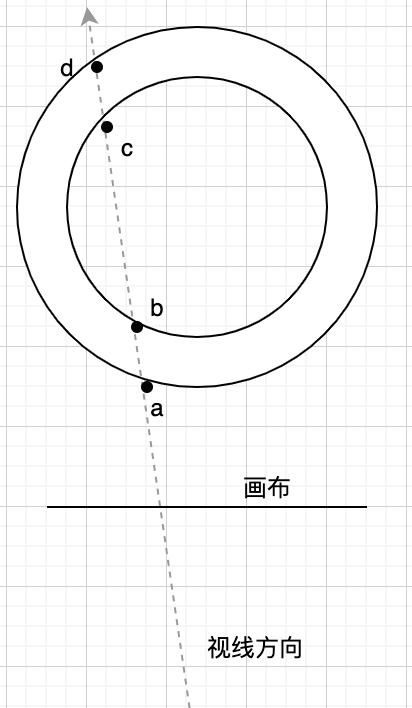
\includegraphics[width=0.3\textwidth]{images/bird-view.png} %插入图片,[]中设置图片大小,{}中是图片文件名
\end{figure}

\subsection{得到像素亮度}

对于圆环上每一像素,其反射的光线强度取决于其在圆环上的位置是否朝向光线。这里假设圆环发生的是漫反射,直接被光线照射的位置亮度最大,而不是像镜面反射那样将光线反射进视线最多的区域亮度最高$^{[2]}$

算法实现为:对于每一2.2中过滤后的所有像素,其在圆环上占的一小块区域可以看做一个平面。对于这些平面,得到垂直于平面的向量,和光线向量得到点乘结果。

\quad 点乘结果为正值,代表向量和光线在同一直线上,方向相同。可以判断像素是背光的像素,没有被光线照射,类似于俯视图中的b d点

\quad 点乘结果为0,代表向量和光线垂直,则平面几乎没有被光线照射,亮度为0

\quad 点乘结果为负值,代表向量和光线相逆,平面正对光线。则点乘结果绝对值越大,平面越被光线直射,亮度越大

得到亮度数值后,每一数值被对应到一个字符,使用的字符包含.,-;=!*\#\$@,选取这些字符的依据是笔画多少。例如字符@拥有较多笔画,则对应亮度较大的像素

\subsection{旋转圆环}

为了得到一个不断变化的圆环图像,程序每0.1秒对每一像素延y = 100, z = 1000 的直线翻转(即令圆环在原位置沿x轴翻转)。翻转后重新进入2.2将圆环映射进二维画布,得到亮度,输出到终端

\subsection{更新终端输出}

经过2.4,程序已经得到一个长宽对应画布大小的矩阵。矩阵中每一个元素为一个字符代表像素亮度。为了在终端打印这个矩阵,并在经过2.5中翻转后更新终端中的矩阵,程序使用python包curses不断刷新输出。


\section{Reference}
\noindent $[1] https://www.youtube.com/watch?v=sW9npZVpiMI&t=100s$\\
$[2] https://materials.doc.ic.ac.uk/resources/2021/60005$\\
$[3] https://docs.python.org/3/howto/curses.html$





\end{document}
